As mentioned in Section \ref{sec:Simulations}, the measurements on Higgs cross sections (Inclusive and differential) are made in a fiducial region that matches the reconstruction level selection. % in order to minimize the effects of model depedence.
%in order to reduce the effects of model dependent acceptances. 
%Fiducial selection mimics the reconstruction level selection, 
%which is optimized to detect a low mass Higgs ($m_{H}$ 125 $\GeV$) boson decaying to 4 
%leptons through a pair of Z bosons. 
Measurement strategy and definition of the fiducial volume is optimized to:
\begin{itemize}
	\item detect a low mass Higgs ($m_{H}$ 125.09 $\GeV$) boson decaying to 4 leptons through a pair of Z bosons
	\item keep the measurements independent of how the Higgs boson is produced. 
\end{itemize}

For reconstruction efficiency to be independent of fiducial phase space, it is necessary to include isolation in the definition of fiducial phase space. % to make the reconstruction efficiencies independent of fiducial phase space.
%independent of the number of jets.
\par
In case of associated production of Higgs with vector bosons where the bosons can decay leptonically, there is possibility that Higgs is reconstructed from wrong combination of leptons. 
%In sub-leading SM production modes there can be associated vector bosons which can decay to leptons, and therefore the reconstructed Higgs 
%boson candidate may not be composed of the correct combination of the leptons. 
This makes it necessary to consider such ``wrong combination'' events as a background in order to keep complete information from unbinned simultaneous fit of signal and background parameterizations to four-lepton invariant mass.
%
%In order to retain the full information from an unbinned simultaneous fit of the
%signal and the background PDFs to the four-lepton distribution of invariant mass, it is necessary to treat such ``wrong combination'' events as a background.
\par
%Further signal-induced background can be formed due to imperfect correspondence between quantities at particle level and corresponding quantities at the reconstruction level. 
Also, signal events which pass the fiducial level selections but fail the reconstruction are accounted  in the fiducial efficiency
($\epsilon$) and the events which pass the reconstruction but fail the fiducial selections are referred to as ``nonfiducial signal'' events ($f_{nonfid}$) and are treated as a background as illustrated in Figure \ref{fig:cartoon} \cite{fid_diagram}.

%==================
\begin{figure}[!h!tb]
 \begin{center}
    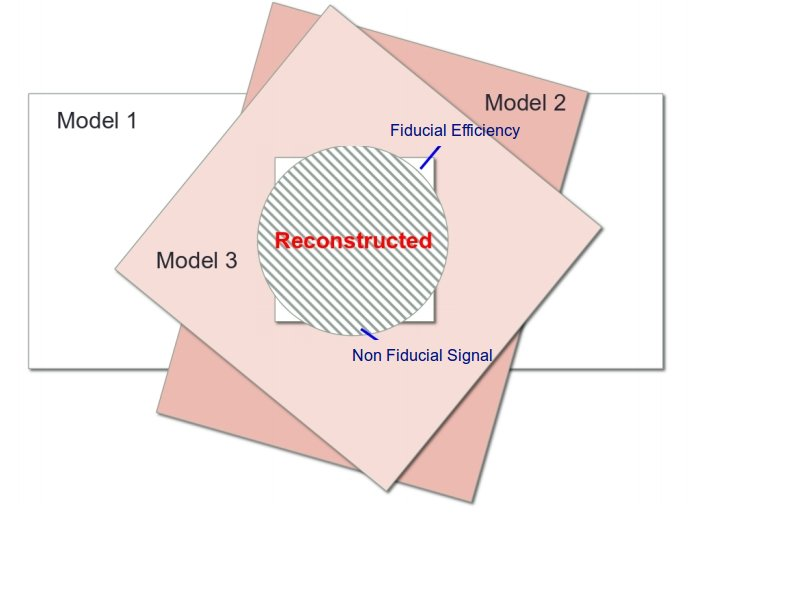
\includegraphics[width=0.65\textwidth,angle=0]{Figures/cartoon.jpg}
    \caption{Fiducial efficiency($\epsilon$) and nonfiducial($f_{nonfid}$) signal definition.}
 \label{fig:cartoon}
 \end{center}
\end{figure}

%==================

\par
There is significant effect of imperfect resolution of the detector on the differential measurements particularly in case of jet related observables for which detector resolution is poor. A procedure, called unfolding, is applied for the correction of the reconstruction efficiencies and the effects are applied to the measurements. %This is known as unfolding. 

The effects of imperfect detector resolution can in general have a non-negligible effect on shape of the distributions of measured observables. 
For this reason, for differential cross section measurements of Higgs, a procedure to correct the detection efficiencies and resolution effects is 
applied. \\
The details of the procedure would be described in next Sections.
%Throughout this document, this procedure will be referred to as the unfolding procedure, and the unfolded differential distributions will be referred to as 
%distributions at the fiducial level.
%The reconstruction level selection, fiducial phase space definition, statistical procedure, and their model dependence will be described in the subsequent Sections.
